% generated by scripts/pkl_to_latex.py
% source PKL : tscan_v1_L8_Ne8_U5_mode-uniform_nmin2_solver-gcg_full_es_restarts8_iter200_kmax4_tol1em09_t0.05to2_N20-d03538a42051.pkl
% scan type  : tscan
% state      : ex_singlet
% requires   : \usepackage{pgfplots} \pgfplotsset{compat=1.18}
% colours match the matplotlib PDF (tab10 cycle)
\definecolor{gmeC0}{HTML}{1F77B4}
\definecolor{gmeC1}{HTML}{FF7F0E}
\definecolor{gmeC2}{HTML}{2CA02C}
\definecolor{gmeC3}{HTML}{D62728}
\definecolor{gmeC4}{HTML}{9467BD}
\definecolor{gmeC5}{HTML}{8C564B}
\definecolor{gmeC6}{HTML}{E377C2}
\definecolor{gmeC7}{HTML}{17BECF}

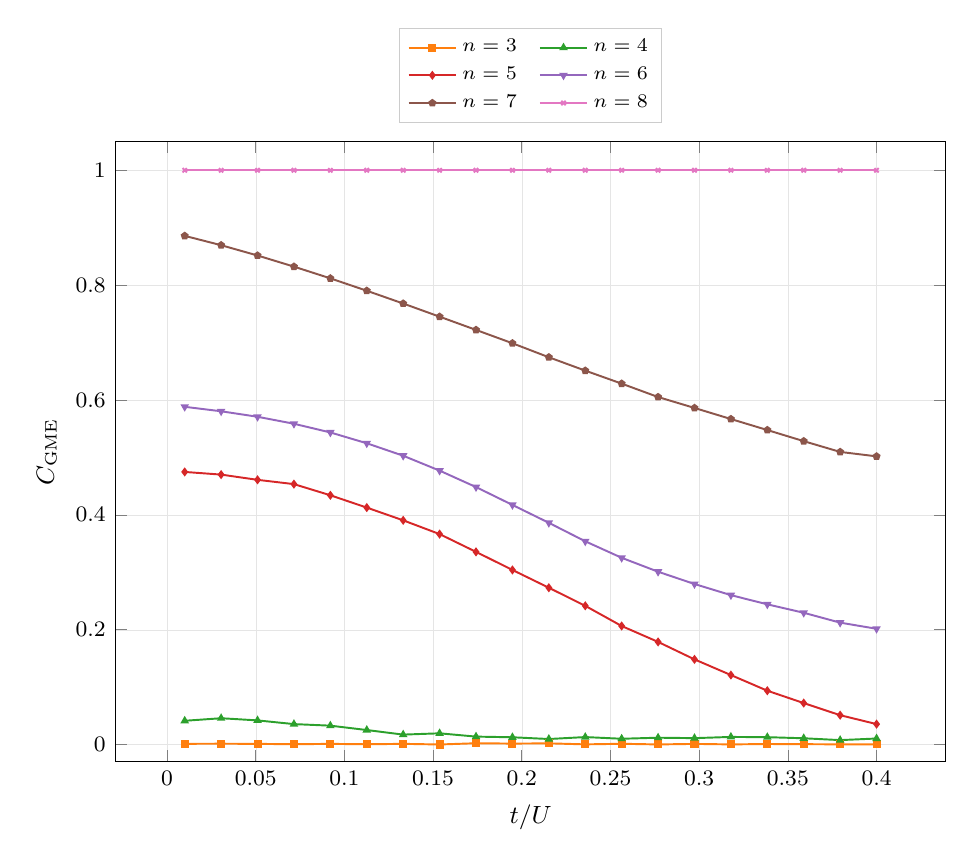
\begin{tikzpicture}
  \begin{axis}[
    width=\columnwidth,
    height=0.78\columnwidth,
    xlabel={$t/U$},
    ylabel={$C_{\mathrm{GME}}$},
    grid=both,
    grid style={line width=.1pt, draw=gray!20},
    tick label style={font=\footnotesize\rmfamily, /pgf/number format/fixed},
    label style={font=\small\rmfamily},
    scaled ticks=false,
    legend style={font=\scriptsize\rmfamily, draw=gray!40, at={(0.5,1.03)}, anchor=south, /tikz/every even column/.append style={column sep=6pt}},
    legend cell align={left},
    legend columns=2,
    ymin=-0.03,
    ymax=1.05,
  ]
    \addplot[color=gmeC1, mark=square*, mark size=1.1pt, line width=0.7pt] coordinates {
        (0.01,0.001205) (0.030526,0.001426) (0.051053,0.001098) (0.071579,0.000515)
        (0.092105,0.001112) (0.112632,0.000439) (0.133158,0.001156) (0.153684,0.000047)
        (0.174211,0.002222) (0.194737,0.001601) (0.215263,0.00202) (0.235789,0.000274)
        (0.256316,0.001269) (0.276842,0.000134) (0.297368,0.001059) (0.317895,0.000183)
        (0.338421,0.000887) (0.358947,0.000606) (0.379474,0.000251) (0.4,0.000067)
    };
    \addlegendentry{$n=3$}
    \addplot[color=gmeC2, mark=triangle*, mark size=1.1pt, line width=0.7pt] coordinates {
        (0.01,0.041324) (0.030526,0.045777) (0.051053,0.041996) (0.071579,0.035549)
        (0.092105,0.032828) (0.112632,0.025211) (0.133158,0.017263) (0.153684,0.019495)
        (0.174211,0.013764) (0.194737,0.012614) (0.215263,0.009574) (0.235789,0.012972)
        (0.256316,0.010032) (0.276842,0.011848) (0.297368,0.011108) (0.317895,0.013206)
        (0.338421,0.012774) (0.358947,0.010882) (0.379474,0.007664) (0.4,0.010451)
    };
    \addlegendentry{$n=4$}
    \addplot[color=gmeC3, mark=diamond*, mark size=1.1pt, line width=0.7pt] coordinates {
        (0.01,0.474673) (0.030526,0.470044) (0.051053,0.460923) (0.071579,0.453456)
        (0.092105,0.434028) (0.112632,0.412586) (0.133158,0.390391) (0.153684,0.366435)
        (0.174211,0.33547) (0.194737,0.303991) (0.215263,0.272998) (0.235789,0.241512)
        (0.256316,0.206361) (0.276842,0.178678) (0.297368,0.148245) (0.317895,0.120981)
        (0.338421,0.093685) (0.358947,0.072143) (0.379474,0.051068) (0.4,0.03555)
    };
    \addlegendentry{$n=5$}
    \addplot[color=gmeC4, mark=triangle*, mark size=1.1pt, mark options={rotate=180}, line width=0.7pt] coordinates {
        (0.01,0.588094) (0.030526,0.580308) (0.051053,0.570748) (0.071579,0.558567)
        (0.092105,0.543451) (0.112632,0.52461) (0.133158,0.502901) (0.153684,0.476956)
        (0.174211,0.44833) (0.194737,0.417216) (0.215263,0.386096) (0.235789,0.353888)
        (0.256316,0.325154) (0.276842,0.30089) (0.297368,0.279511) (0.317895,0.260133)
        (0.338421,0.244119) (0.358947,0.22943) (0.379474,0.212215) (0.4,0.20156)
    };
    \addlegendentry{$n=6$}
    \addplot[color=gmeC5, mark=pentagon*, mark size=1.1pt, line width=0.7pt] coordinates {
        (0.01,0.885815) (0.030526,0.869529) (0.051053,0.851579) (0.071579,0.832215)
        (0.092105,0.811782) (0.112632,0.790214) (0.133158,0.767948) (0.153684,0.745037)
        (0.174211,0.722003) (0.194737,0.698769) (0.215263,0.674372) (0.235789,0.651087)
        (0.256316,0.628442) (0.276842,0.60514) (0.297368,0.586099) (0.317895,0.566816)
        (0.338421,0.547631) (0.358947,0.528266) (0.379474,0.509533) (0.4,0.501796)
    };
    \addlegendentry{$n=7$}
    \addplot[color=gmeC6, mark=x, mark size=1.1pt, line width=0.7pt] coordinates {
        (0.01,1) (0.030526,1) (0.051053,1) (0.071579,1)
        (0.092105,1) (0.112632,1) (0.133158,1) (0.153684,1)
        (0.174211,1) (0.194737,1) (0.215263,1) (0.235789,1)
        (0.256316,1) (0.276842,1) (0.297368,1) (0.317895,1)
        (0.338421,1) (0.358947,1) (0.379474,1) (0.4,1)
    };
    \addlegendentry{$n=8$}
  \end{axis}
\end{tikzpicture}
